\section{Thuật toán Horspool}

\subsection{Đặc điểm chính}

Thuật toán Horspool là một phiên bản đơn giản hóa của thuật toán Boyer-Moore. Thuật toán được đề xuất bởi R. Nigel Horspool, với mục tiêu giữ lại phần hiệu quả nhất của Boyer-Moore nhưng làm cho cách cài đặt trở nên đơn giản hơn.

Thay vì sử dụng đầy đủ cả hai heuristic như Boyer-Moore, Horspool chỉ sử dụng phép dịch chuyển bad-character dựa trên ký tự ngoài cùng bên phải của cửa sổ văn bản. Nhờ đó, thuật toán rất dễ cài đặt và thường có hiệu năng tốt trong thực tế, đặc biệt khi bảng chữ cái lớn so với độ dài mẫu, chẳng hạn như các tìm kiếm thông thường trên văn bản ASCII.

Thuật toán có các đặc điểm sau:

\begin{itemize}
    \item là phiên bản đơn giản hóa của thuật toán Boyer-Moore;
    \item dễ cài đặt;
    \item giai đoạn tiền xử lý có độ phức tạp thời gian \(O(m+\sigma)\) và không gian \(O(\sigma)\);
    \item giai đoạn tìm kiếm có độ phức tạp thời gian \(O(mn)\);
    \item số phép so sánh trung bình trên một ký tự văn bản nằm trong khoảng từ \(\frac{1}{\sigma}\) đến \(\frac{2}{\sigma+1}\).
\end{itemize}

\subsection{Mô tả thuật toán}

Phép dịch chuyển bad-character được sử dụng trong thuật toán Boyer-Moore không thực sự hiệu quả với bảng chữ cái nhỏ. Tuy nhiên, khi kích thước bảng chữ cái lớn so với độ dài mẫu, ví dụ như bảng mã ASCII trong các thao tác tìm kiếm văn bản thông thường, phép dịch chuyển này trở nên rất hữu ích.

Việc chỉ sử dụng riêng phép dịch chuyển bad-character tạo ra một thuật toán có hiệu năng rất tốt trong thực tế. Horspool đề xuất chỉ dùng phép dịch chuyển bad-character của ký tự ngoài cùng bên phải trong cửa sổ văn bản để tính khoảng dịch chuyển của mẫu trong thuật toán Boyer-Moore.

Giai đoạn tiền xử lý có độ phức tạp thời gian \(O(m+\sigma)\) và độ phức tạp không gian \(O(\sigma)\).

Giai đoạn tìm kiếm có độ phức tạp bậc hai trong trường hợp xấu nhất. Tuy nhiên, có thể chứng minh rằng số phép so sánh trung bình trên một ký tự văn bản nằm trong khoảng:

\[
\frac{1}{\sigma}
\quad \text{đến} \quad
\frac{2}{\sigma+1}.
\]

\subsection{Cài đặt bằng C++}
\begin{verbatim}
#include <iostream>
#include <vector>
#include <string>
#include <cstring>

using namespace std;

const int ASIZE = 256;

/* Bad Character Shift Table */
void preBmBc(const string &pat, vector<int> &bmBc) {
    int m = pat.length();

    bmBc.assign(ASIZE, m);

    for (int i = 0; i < m - 1; ++i) {
        bmBc[(unsigned char)pat[i]] = m - 1 - i;
    }
}

/* Horspool Algorithm */
void Horspool(const string &pat, const string &txt) {
    int m = pat.length();
    int n = txt.length();

    if (m == 0 || n < m) {
        return;
    }

    vector<int> bmBc;

    /* Preprocessing */
    preBmBc(pat, bmBc);

    /* Searching */
    int j = 0;

    while (j <= n - m) {
        unsigned char c = (unsigned char)txt[j + m - 1];

        if (pat[m - 1] == txt[j + m - 1] &&
            memcmp(pat.c_str(), txt.c_str() + j, m - 1) == 0) {
            cout << "Pattern found at index: " << j << endl;
        }

        j += bmBc[c];
    }
}

int main() {
    string text = "ABAAABCDABCABC";
    string pattern = "ABC";

    Horspool(pattern, text);

    return 0;
}
\end{verbatim}

\subsection{Kiểm nghiệm thuật toán}

\textbf{Pha tiền xử lý:}

\begin{figure}[H]
    \centering
    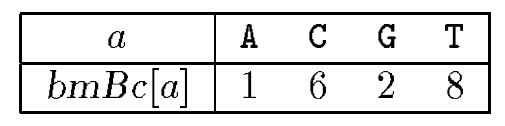
\includegraphics[width=10cm]{Images/2026-05-18-15-44-06.png}
    \caption{Kết quả tiền xử lý bảng bmBc của thuật toán Horspool}
    \label{fig:horspool-preprocess}
\end{figure}

Bảng $bmBc$ được sử dụng bởi thuật toán Horspool

\textbf{Pha tìm kiếm:}

Lần 1: 

\begin{figure}[H]
    \centering
    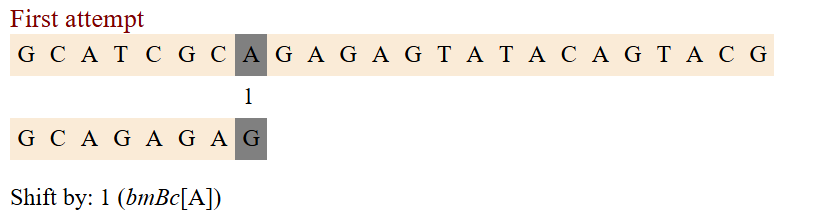
\includegraphics[width=15cm]{Images/2026-05-18-15-45-39.png}
    \caption{Bước 1 trong quá trình thực hiện thuật toán Horspool}
    \label{fig:horspool-step-1}
\end{figure}

Lần 2: 

\begin{figure}[H]
    \centering
    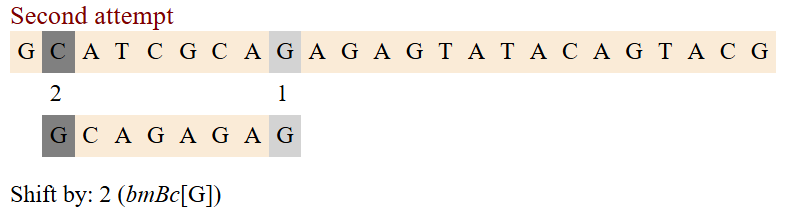
\includegraphics[width=15cm]{Images/2026-05-18-15-45-50.png}
    \caption{Bước 2 trong quá trình thực hiện thuật toán Horspool}
    \label{fig:horspool-step-2}
\end{figure}

Lần 3: 

\begin{figure}[H]
    \centering
    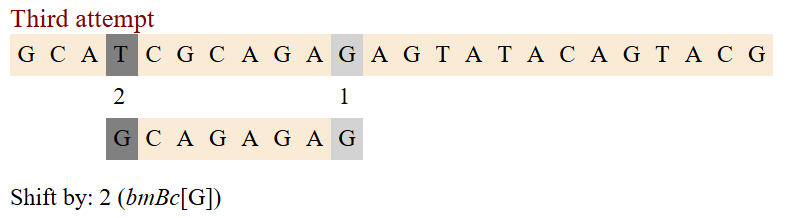
\includegraphics[width=15cm]{Images/2026-05-18-15-46-00.png}
    \caption{Bước 3 trong quá trình thực hiện thuật toán Horspool}
    \label{fig:horspool-step-3}
\end{figure}

Lần 4: 

\begin{figure}[H]
    \centering
    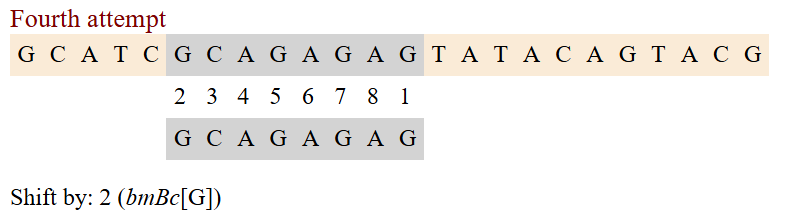
\includegraphics[width=15cm]{Images/2026-05-18-15-46-08.png}
    \caption{Bước 4 trong quá trình thực hiện thuật toán Horspool}
    \label{fig:horspool-step-4}
\end{figure}

Lần 5: 

\begin{figure}[H]
    \centering
    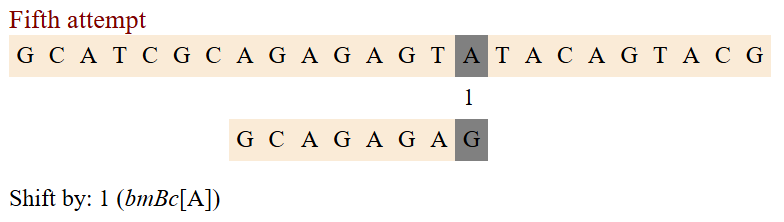
\includegraphics[width=15cm]{Images/2026-05-18-15-46-20.png}
    \caption{Bước 5 trong quá trình thực hiện thuật toán Horspool}
    \label{fig:horspool-step-5}
\end{figure}

Lần 6: 

\begin{figure}[H]
    \centering
    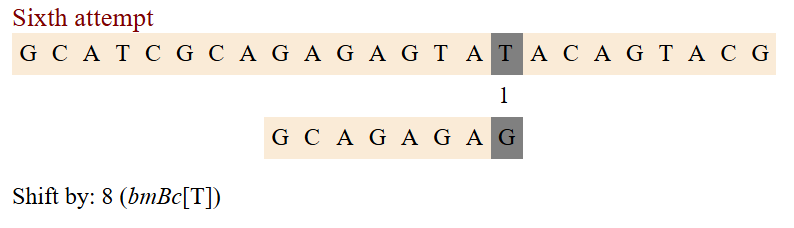
\includegraphics[width=15cm]{Images/2026-05-18-15-46-32.png}
    \caption{Bước 6 trong quá trình thực hiện thuật toán Horspool}
    \label{fig:horspool-step-6}
\end{figure}

Lần 7: 

\begin{figure}[H]
    \centering
    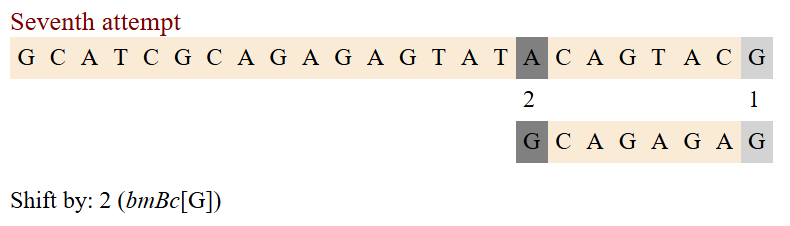
\includegraphics[width=15cm]{Images/2026-05-18-15-46-40.png}
    \caption{Bước 7 trong quá trình thực hiện thuật toán Horspool}
    \label{fig:horspool-step-7}
\end{figure}

Thuật toán Horspool thực hiện 17 lần so khớp chuỗi trong ví dụ trên.